% simple document template
\documentclass[12pt]{article}
\usepackage{tikz}
\usetikzlibrary{graphs}
\usetikzlibrary {mindmap}
\usepackage{hyperref}
\begin{document}

\title{Flips Websites}
\author{Pengfei}
\date{\today}
\maketitle

\tableofcontents

% /usr/local/texlive/2023/bin/universal-darwin/pdftex
% /usr/local/texlive/2023/texmf-var/web2c/pdftex
% /usr/local/texlive/2023/texmf-var/fonts/map/pdftex
% /usr/local/texlive/2023/bin/universal-darwin/pdftex
% /usr/local/texlive/2023/texmf-dist/tex/generic/pdftex
% ==========[Section Potential]===========
\section{Potential}
\subsection{ROI}
\paragraph{How many websites}~\\
\begin{verbatim}
    1. 1B websites
    2. 2B houses
    3. 7B videos on tictoc
\end{verbatim}

\subsection{Goal}
\begin{itemize}
    \item 1. 2024: make \$1000 to by a mac book air M3 chips
\end{itemize}

\subsection{How to make it work}
\begin{itemize}
    \item 1. Keyword choice and SEO
    \item 2. Focus on keywords solve real problems
    \item 3. Find a keyword:
    \item 4. low competition good search vol and solve real problems
    \item 5. Make more sites to blank page 1 of google
    \item 6. Bad things happen: depend on google algorithm
    \item 7. Make a website
\end{itemize}

\subsection{Flip markets}

Takes ~15\% fee
\begin{itemize}
    \item 1. Lead Spring
    \item 2. \href{https://flippa.com/}{Flippa}
    \item 3. Flip content
    \item 4. Flip videos
\end{itemize}

\subsection{Google}
\paragraph{Google search trends}~\\

\begin{figure}
    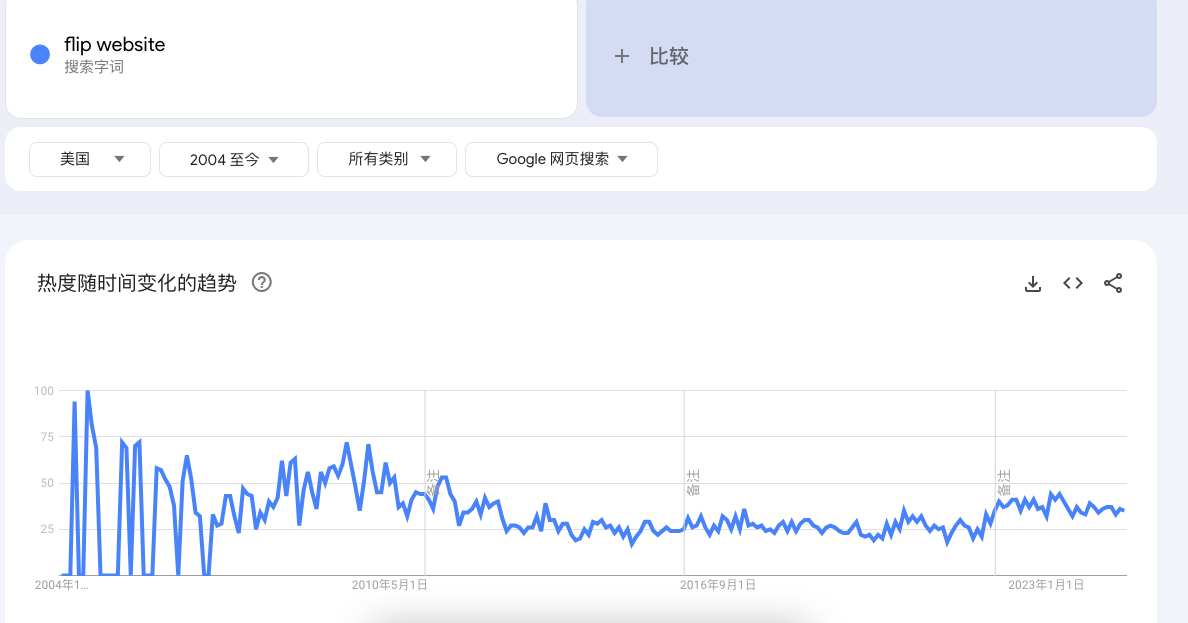
\includegraphics[width=0.5\textwidth]{./images/trend_flip_websites.png}
    \caption{Google search trends}
\end{figure}

Key findings:
\begin{itemize}
    \item 1. gradually increases
    \item 2. every 6 years major update to google
\end{itemize}

\subsection{Example}
\paragraph{Ideas}~\\

Guidance: some topic I am interested or some digital product I can improve

\begin{itemize}

    \item \href{https://www.mybabyboutique.us/}{MyBaby.com}
    \item \href{https://www.printable-ruler.net/}{Printable Ruler(I can customize the rulers!)}
\end{itemize}


% ==========[Section References]===========
\section{References}
\subsection{Web}
\begin{itemize}
    \item 1. \href{https://www.youtube.com/watch?v=UaJIkkZbaEY}{Matt Diggity}
    \item 2. \href{https://jaserodley.com/website-flipping/}{Jase Rodley}
\end{itemize}
    
\end{document}